\chapter{Methodology}\label{ch:methodology}

Data Quality methodology consists of two main parts, the model and the metamodel.
The model defines activities, their description, goals and sequence of order needed for extraction of Data Quality metrics.
The metamodel defines components of DQ process, maps the relationship among the components and activities respectively.

\section{Data Quality and Security}

In addition to model and architecture security mechanism, we have to consider security of data sets.
Data often contains personal information of users - so called \textit{sensitive attributes}.
Such information can be in a~form of personal identifiers or quasi-identifiers.
\textit{Personal identifier} is an unique information that identifies a~user - a~birth number, bank account number and other types of personal IDs.
\textit{Quasi-identifiers} are characteristics which needs to be used in combination with others to identify an entity - examples are gender, postal code, age or nationality.

To prevent data stealing and following re-identification of users, several models exists to protect personal information of individuals in dataset.
Those privacy models are \textbf{optimal k-anonymity}, \textbf{l-diversity}, \textbf{t-closeness} and \textbf{differential privacy}.
Three general types of attack to datasets exists:
\begin{enumerate*}[label=(\roman*)]
    \item \label{itm:reident} re-identifying an individual,
    \item \label{itm:query} query whether an individual is a~member of a~dataset,
    \item \label{itm:linking} linking an individual to a~sensitive attribute.
\end{enumerate*}

\textbf{Optimal k-anonymity} protects against both cases~\ref{itm:reident} and~\ref{itm:query} by transforming quasi-identifiers so that at least \( k - 1 \) members of set are indistinguishable from each other - group based anonymization.
Identifiers are transformed by suppression (needless attributes are replaced with \textit{dummy} values) and generalization (individual values of attributes are replaced with a~broader category - e.g.\ specific age can be replaced by a~range).
As \( k \) increases risk of data exploit reduces, on the other hand data quality decreases - we are talking about a~\textit{privacy-utility} tradeoff.
Moreover, the \( k \) is limit - in order for this method to work if \( k \) is set to \( k \triangleq 10 \) then any group must contain at least \( 10 \) individuals.
The first drawback of k-anonymity is vulnerability to \textit{homogeneity attack} which works on premise of data having sensitive value identical within a~set of \( k \) records - it is enough to find the group of records, the individual belongs to, if all of them have the same sensitive value.
Second drawback is the possibility of \textit{background knowledge attack} where attacker identifies associations among one or more quasi-identifiers and reduces the set of possible values for the sensitive attribute.

Both \textbf{l-diversity} and \textbf{t-closeness} are group based anonymization techniques building on a~concept of \textbf{optimal k-anonymity}.
In addition to \textbf{optimal k-anonymity}, \textbf{T-closeness} transforms quasi-identifiers such that each group is within a~distance \( t \) of the distribution of sensitive values for the entire dataset~\cite{web:privacy-models}.
The distance is measured as the cumulative absolute difference of the distributions, as \( t \) decreases both risk of sensitive attribute disclosure and data quality decreases.
Suppose that the sensitive attribute is salary.
Each group's frequency distribution of salary will be within a~distance \( t \) from the salary frequency distribution for the entire dataset~\cite{web:privacy-models}.

\textbf{Differential privacy} and its variants (epsilon, epsilon-delta) are statistical techniques aiming to protect data against \textit{differentiated attack}.
The model guarantees that even if someone has complete information about 99 of 100 people in a~data set, they still cannot deduce the sensitive information about the final person~\cite{web:differential-privacy}.
The mechanism works by adding random noise to the aggregate data, leaving only a~trend without possibility to figure out exact values in data (e.g.\ information that \( n\% \) of users prefer some product over another).

\section{Business Problems and Data Defects}

% Není možné mluvit o kvalitě dat a metodikách pro její zajištění, bez zmínky o konkrétních typech problémů, které se v rámci tématu vyskytují.
It is not possible to talk about data quality and methodologies for ensuring it, without mentioning the specific types of problems that occur within the topic.
There is quite a few common defects in the field of data engineering and data science.

\subsection*{Missing Data}

This is data that does not reach the destination data store.
This problem usually occurs when handling the data needed to clean up in the source database; by operating with invalid or incorrect lookup table in the transformation logic; or by invalid table joins.

\paragraph*{Example} We transform data from Task Management Solution.
Lookup table should contain a field value of \enquote{Minor} which maps to \enquote{Low}.
However, source data field contains \enquote{Mino} - missing the \textit{r} and fails the lookup, resulting in the target data field containing null.
If this occurs on a key field, a possible join would be missed and the entire row could fall out.

\subsection*{Truncation of Data}

Many data is being lost by truncation of the data fields.
This happens when there are invalid field lengths on target database or by transformation logic not taking into account field lengths from the source.

\paragraph*{Example} We transform financial data with complete exchange-traded fund (ETF) names.
Source field value \enquote{iShares Global High Yield Corp Bond UCITS ETF} is being truncated to \textit{varchar(32)}.
since the source data field did not have the correct length to capture the entire field, only \enquote{iShares Global High Yield Corp B} is stored.

\subsection*{Data Type Mismatch}

Data types not setup correctly on target database cause serious problems.
This usually happens when using ETL pipeline with an automatic or semi-automatic column type recognition.
% Data inženýr spoléhá na bezchybné rozpoznání datového typu a nezkontroluje správnost výstupních tabulek.
The data engineer relies on error-free data type recognition and does not check the accuracy of the output tables.

\paragraph*{Example} Source data field was required to be a \textit{varchar}, however, when initially configured, was setup as a \textit{date}.

\subsection*{Null Translation}

In the source dataset, \textit{null} values are not being transformed to correct target values.
Development team did not include the \textit{null} translation in the ETL process.

\paragraph*{Example} A \enquote{Null} source data field was supposed to be transformed to \enquote{None} in the target data field.
However, the logic was not implemented, resulting in the target data field containing \enquote{null} values\footnotemark.

\footnotetext{
    None is a concept that describes the absence of anything at all (nothingness), while Null means \textit{unknown} (we do not know if there is a value or not).
}

\subsection*{Wrong Translation}

Wrong translations happen when a source data field for \textit{null} was supposed to be transformed to \enquote{None} in the target data field, but was not transformed correctly.
The logic was not implemented, resulting in the target data field containing \textit{null} values.
Wrong translation is the exact opposite to \textit{Null Translation}.

\paragraph*{Example} Target field should only be populated when the source field contains certain values, otherwise should be set to null.
Let's look at a very basic example.
During analytical processing of medical data (e.g., list of patients with oncological finding), we need to set target field to \textit{true} if the one or multiple source values indicate certain treatment.
However, the target field is populated (either with blank charater or other values) although source values do not correspond to the required logic.

\subsection*{Misplaced Data}

If the source data fields are not being transformed to the correct target data fields, we call the issue \enquote{Misplaced Data}.
One of the possible causes is that development team inadvertently mapped the source data field to the wrong target data field.

\paragraph*{Example} A source data field was supposed to be transformed to target data field \enquote{Last\_Update}.
However, the development team inadvertently mapped the source data field to \enquote{Date\_Created}.

\subsection*{Extra Records}

Records which should be excluded in the ETL are included in the ETL.
This happens when developers do not include filter in their code.

\paragraph*{Example} If a record has the deleted field populated, the record and any data related to that record should not be in any ETL.

\subsection*{Not Enough Records}

Records which should be in the ETL are not included in the ETL.
Development team had a filter in their code which should not have been there.

\paragraph*{Example} If a record was in a certain state, it should be sent through ETL pipeline over to the data warehouse.

\subsection*{Transformation Logic Errors}

Testing sometimes can lead to finding \enquote{holes} in the transformation logic or realizing the logic is unclear.

Sometimes, the processes are just way too complicated and development team does not take into account special cases.
Most cases fall into a certain branch of logic for a transformation, but a small subset of cases (sometimes with unusual data) may not fall into any branches.
How the analytics and developers handles these cases could be different (and may both end up being wrong) and the logic is changed to accommodate the cases.
The next reason why this happens is that analytic and developer have different interpretation of transformation logic, which results in different values.
This leads to the logic being re-written to become clearer.

\paragraph*{Example} International cities that contain special language specific characters might need to be dealt with in the ETL code (e.g., Århus).

\subsection*{Simple and small Errors}

Capitalization, spacing and other small errors cause problems with data.
Data inconsistencies are easy to fix, but happen often.
The only real solution is to always double check data and ETL procedure.

\subsection*{Sequence Generator}

Ensuring that the sequence number of reports are in the correct order is very important when processing follow up reports or answering to an audit.
If the sequence generator is not configured correctly, procedure results in records with a duplicate sequence number.

\paragraph*{Example} Duplicate records in the sales report were doubling up several sales transactions which skewed the report significantly.

\subsection*{Undocumented Requirements}

During ETL development, sometimes certain requirements are found, that are \enquote{understood} but are not actually documented anywhere.
This causes issues when members of the development team do not understand or misunderstood the undocumented requirements.

\paragraph*{Example} ETL pipeline contains a restriction in the \enquote{where} clause, limiting how certain reports are brought over.
Moreover, there were used mappings that were understood to be necessary, but were not actually in the requirements.
Occasionally, it turns out that the understood requirements are not what the business wanted.

\subsection*{Duplicate Records}

Duplicate records are two or more records that contain the same data.
This issue happens when development team does not add the appropriate code to filter out duplicate records or there is some unexpected error in data generators.

\paragraph*{Example} Duplicate records in the sales report were doubling up several sales transactions which skewed the report significantly.

\subsection*{Numeric Field Precision}

Numbers that are not formatted to the correct decimal point or not rounded per specifications cause precision problems.
This has several causes, development team rounded the numbers to the wrong decimal point, used wrong rounding type or used wrong data type which lead to faulty rounding.

\paragraph*{Example} The sales data did not contain the correct precision and all sales were being rounded to the whole dollar.

\subsection*{Rejected Rows}

Data rows that get rejected by ETL process due to data issues.
Development team did not take into account data conditions that break the ETL for a particular row.

\paragraph*{Example} Missing data rows on the sales table caused major issues with the end of year sales report.

% a~\cite{web:common-defects}

\section{Model}

The methodology has several important components that need to be identified or developed.
The metamodel that covers the required components is as depicted in figure~\ref{fig:methodology-metamodel}.
The activities within the process model have a goal to develop those components.

Overall, the methodology consists of two main processes.
The first one is \textbf{Specification Process}.
The goal of this processs is to identify and define context specific ways to measure data quality.
The second one is an \textbf{Execution Process}.
Its main goal is to \textit{collect} and \textit{verify} data with output from \textit{Specification Process} taken into account.

\begin{figure}[htb]
    \centering
    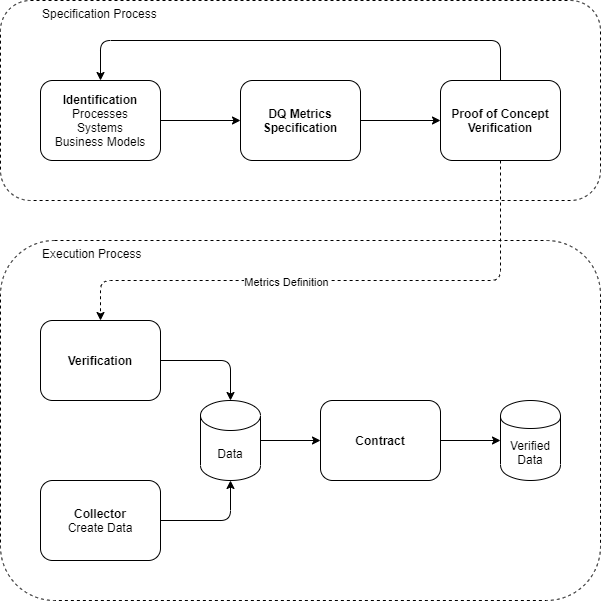
\includegraphics[width=0.7\textwidth]{figures/dq-methodology.png}
    \caption{Methodology Metamodel}
    \label{fig:methodology-metamodel}
\end{figure}
\FloatBarrier

\subsection{Specification Process}

TODO

\subsubsection{Identification}

This activity focuses on identification of systems, processes and business schemes generatig data.
By identifying weak points and bottlenecks in those processes, we can find causes of poor data.
Also, we need to identify the subprocesses or activities that are mostly affected by the product data quality.

\subsubsection{Metrics Specification}

The goal of this activity is to identify the process metrics or KPIs.
Measuring data quality is all about understanding what data quality attributes are and choosing the correct data quality metrics.
Data Quality Attributes were discussed in back in chapter~\ref{ch:related-work} section~\ref{sec:data-quality-attributes} and will be further discussed in chapter~\ref{ch:quality-classification-system}.

\subsubsection{Proof of Concept Verification}

The last part of current process is verification and Proof of Concept.
This activity has to ensure that selected metrics are meaningful enough, capturing the actual condition of data.

\subsection{Execution Process}

TODO

\subsubsection{Collection}

Data collection is a systematic process of gathering observations or measurements.
Data collector can be either \textit{Information System}, computer program or a human.
Before the beginning of collecting data, we need to consider:

\begin{itemize}
    \item the type of data we will collect;
    \item the methods and procedures we will use to collect, store and process data.
\end{itemize}

\subsubsection{Verification}

In our general case, verification is based on actual reliability of data, computed using DQ metrics.
In other scenarios, the verification could be based on data redundancies, therefore based on the comparison of the collected data from two or more different collectors.
If all data match, the data will be considered as valid.
If not, the data remains invalid until a further collector validates it.

Artificial Intelligence and Machine Learning could be used to further ease and optimize data verification.
Especially when processing image data and data with a high level of abstraction.

\subsubsection{Contract}

TODO

\subsection{Supporting Techniques}

TODO

\subsubsection{Proof of Constancy}

Proof of Constant Data, alias Proof of Constancy, is a way to assure a constant accuracy of data.
Data have to be regularly updated to keep the accuracy rate high.
Data accuracy rate will decrease progressively based on a specific time frame basis (e.g., X\% per month).
This percentage is different depending on the type of data.
Data sets more sensitive to changes may see this rate decrease by 5\% to 10\% per month or day depending on the circumstances.
On the other hand, established, well-known sets, will see their rate decrease by 0.1\% per month or even year.
A scale of discount rates will have to be established based on the areas of interest and actual items collected.

\subsubsection{Proof of Trust}

Proof of Trust is an instrument for data collector evaluation.
The collector or generator will get \enquote*{quality score} for his/her or its collection actions.
The more collectors initiate, update and verify data correctly, the higher their \enquote*{quality score} will be.
A higher quality score leads to a higher level of \enquote*{trust}.
On the other hand, incorrect collection leads to a retroactive decrease of the collector's quality score.

\subsection{Roles}

TODO

\section{Use Cases}

In this part, we will present several use cases, to illustrate versatile use of the presented framework.

\subsection{Enterprise Information System}

Enterprises suffer from poor data quality.
We propose, following the methodology, to introduce a central register of data sources.
This central register should be supported by a set of services and a central data repository.

After a thorough analysis of data requirements and their quality, a defined set of metrics and key performance indicators parameterizes the verification chain of activities.
If the predefined quality limit is not met, the data will either be rejected or saved with an error flag.
% Jestliže data splňují požadovanou úrověň chybovosti, projdou kontraktačním procesem a jsou požadována za referenční až do doby, kdy je jejich poslední verze je nařazeným procesem kvalitativně degradována a označena za nedůvěryhodnou.
If the data meets the required level of error, they go through the contracting process and are considered as a reference until their latest version is qualitatively degraded by the ordered process (e.g., Proof of Constancy) and marked as untrusted.

% Penalizací za špatnou kvalitu by bylo automatické hlášení vyššímu managementu společnosti.
A penalty for poor quality would be automatic reporting to the company's senior management.
% Management by následně mohl uvalit na osoby zodpovědné za konkrétní datové sady a datové toky sankce ve formě snížení nebo zrušení osobních odměn.
Management could then impose sanctions on those responsible for specific datasets and data flows in the form of reductions or cancellations of personal rewards.

\subsection{IoT Cluster}

Based on the domain and usage of the IoT devices, the data repository could be either centralized (e.g., nuclear power plant cluster of secondary senzors) or decentralized (e.g., community weather stations).

The verification algorithm would - in this case - consist from two general authorities.
The first authority being \textit{k} nearest neighbours of the same sensors (or IoT devices in general), and the second one being the set of domain rules.
Nearest neighbors provide redundancy by which data can be verified.
A data samotná musí samozřejmě splňovat kriteriální omezení daná doménou využití.

% Špatnou kvalita by vedla ke snížení významnosti senzoru v klusteru, případně jeho dočasnému nebo úplnému vyřazení z provozu.
Poor quality would reduce the importance of the sensor in the cluster, or its temporary or complete decommissioning.
% Tento systém by vytořil i velice účinnou obranou bariéru proti útokům.
This system would also create a very effective defense barrier against attacks, especially against data poisoning.

Data poisoning is a class of attacks on machine learning algorithm where an adversary alters a fraction of the training data in order to impair the intended function of the system.
Objective can be to degrade the overall accuracy of the trained classifier, escaping security detection or to favor one product over the another.
Machine Learning systems are usually retrained after deployment to adapt to changes in input distribution, so data poisoning represents serious danger.

Qualitative degradation of data by Proof of Constancy would not be the so important, because we expect very high update frequency.
However, lower update frequancy of IoT device would suggest an error within a system, which could serve as a warning to network operators about a faulty device.
Data from defective equipment should also not be taken into account in many cases.

\subsection{Open Data Library}

The last Use Case shows usage of completely decentralized solution.
The system would allow those who collect and generate data to be rewarded and data would be accessible for use within a decentralized marketplace.
This decentralized network would democratize access to data while rewarding those who generate it.

Data collection would be done through an application (system) used by a community of collectors who are rewarded for their actions.
This reward is calculated according to a~\enquote*{collection value} price.

The collection value would be calculated using an algorithm that takes into account several criteria, such as:
\begin{itemize}
    \item demand and rarity,
    \item online availability and accessibility,
    \item data licensing market value.
\end{itemize}

Each collector receives a quality score to maintain a high level of reliability
The verified data is then made accessible (through contracting) on the decentralized marketplace and regularly updated to keep it accurate.

Depending on the data, a blockchain could be used as a storage.
Using the blockchain makes the data unalterable, guaranteeing the transparency and traceability of its validation process (collection, verification, update).
The blockchain (tamper-proof, immutable and decentralized) ensures the integrity and verification of the data available on the marketplace.
This brings confidence and security to the data acquirers that exploit it. 
Using \textbf{Smart Contract} technology also guarantees the rewards of the collectors.

Due to the variety of open data, automation of the verification process is practically impossible.
The data must be verified manually.
Thus, a collector has two functions:
\begin{itemize}
    \item initiate the data collection (input and update data),
    \item verify the data collected (check a collected data not yet verified).
\end{itemize}

The mechanism ensures that reward for data collection is divided between collector and verifier.
For example, the collector, who initiated the data, would obtain 60-80\% of the reward.
The verifier would obtain remaining 20-40\%.

\subsubsection{Smart Contracts}

TODO
